\section{Surrogate Loss Function}
\frame{\tableofcontents[currentsection, hideothersubsections]}

\begin{frame}
\frametitle{Surrogate Loss Fn: Intro}

WHAT:\\
handle some \textbf{non}convex problems
by minimizing ``surrogate'' loss functions that are \text{convex}
\vspace{4mm}

WHY:\\
the natural loss function is not convex, e.g.  $0-1$ loss
\vspace{4mm}

HOW:\\
to upper bound the nonconvex loss function by a convex surrogate loss function
that
\begin{itemize}
    \item are convex
    \item upper bounds the original loss.
\end{itemize}
\end{frame}

\begin{frame}
\frametitle{Surrogate Loss Fn: Example}
In the context of learning halfspaces:\\
Hinge loss as a convex surrogate for the $0-1$ loss
\footnote{{\tiny https://scicomp.stackexchange.com/questions/5628/confusion-related-to-convexity-of-0-1-loss-function}}

\begin{figure}
    \centering
    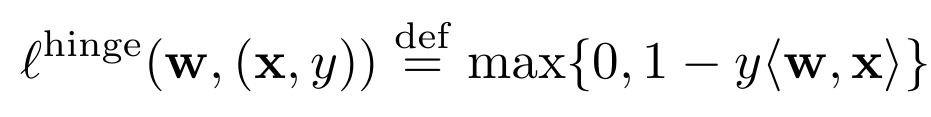
\includegraphics[scale=0.25]{eq_hinge_loss}
\end{figure}

\begin{figure}
    \centering
    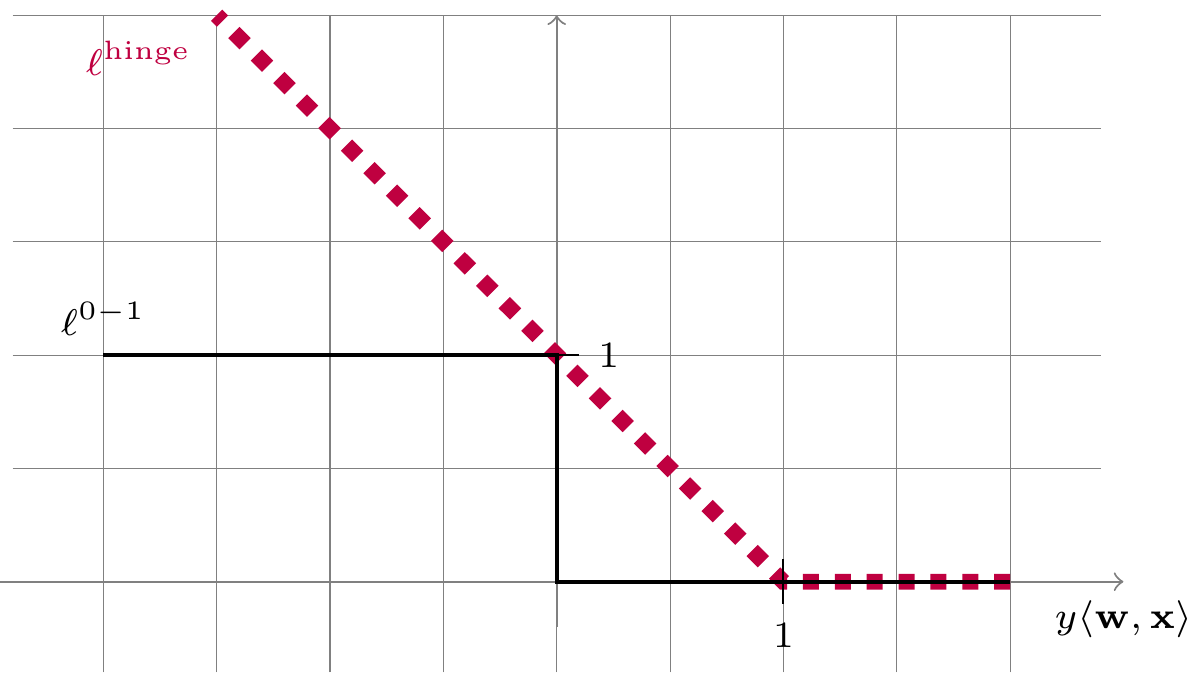
\includegraphics[scale=0.25]{fig_surr_fn}
\end{figure}

\end{frame}



